\documentclass[11pt,a4paper]{article}

\usepackage[utf8]{inputenc}
\usepackage[T1]{fontenc}
\usepackage[spanish,es-tabla,es-nodecimaldot,es-noquoting]{babel}
\usepackage{lmodern}
\usepackage{microtype}
\usepackage[margin=2.4cm]{geometry}
\usepackage{graphicx}
\usepackage{xcolor}
\usepackage{tabularx,booktabs,array}
\usepackage{enumitem}
\usepackage{float}
\usepackage{caption}
\usepackage{pdflscape}
\usepackage{fancyhdr}
\usepackage{titlesec}
\usepackage{listings}
\usepackage[most]{tcolorbox}
\usepackage{tikz}
\usetikzlibrary{positioning,arrows.meta,fit,backgrounds,calc,babel}
\usepackage[hidelinks]{hyperref}
\usepackage{xurl}

% Colores
% Mismos tokens que el sistema de diseño (figma/build.py)
\definecolor{bosque}{HTML}{0B3B2C}
\definecolor{verde}{HTML}{136B4A}
\definecolor{lima}{HTML}{E4F56A}
\definecolor{crema}{HTML}{F7F3EC}
\definecolor{tinta}{HTML}{16211C}
\definecolor{gris}{HTML}{5F6B64}
\definecolor{linea}{HTML}{E7E1D6}
\definecolor{ambar}{HTML}{FFF3D6}

\graphicspath{{../figma/png/}{img/}}

\titleformat{\section}{\Large\bfseries\color{bosque}}{\thesection.}{0.6em}{}
\titleformat{\subsection}{\large\bfseries\color{tinta}}{\thesubsection.}{0.6em}{}
\titleformat{\subsubsection}{\normalsize\bfseries\color{verde}}{}{0em}{}

\pagestyle{fancy}
\fancyhf{}
\fancyhead[L]{\small\color{gris}Take a Break · Preentrega}
\fancyhead[R]{\small\color{gris}Desarrollo de Aplicaciones I · UADE}
\fancyfoot[C]{\small\thepage}
\renewcommand{\headrulewidth}{0.4pt}

\setlist{itemsep=2pt,topsep=4pt}
\setlength{\parskip}{0.5em}
\setlength{\parindent}{0pt}
\renewcommand{\arraystretch}{1.25}
\newcolumntype{L}{>{\raggedright\arraybackslash}X}

\lstset{basicstyle=\ttfamily\small,frame=single,rulecolor=\color{linea},
  backgroundcolor=\color{crema},xleftmargin=4pt,xrightmargin=4pt,columns=fullflexible,
  literate={á}{{\'a}}1 {é}{{\'e}}1 {í}{{\'i}}1 {ó}{{\'o}}1 {ú}{{\'u}}1 {ñ}{{\~n}}1}

% Requisito funcional
\newtcolorbox{rf}[1]{enhanced,colback=white,colframe=bosque,coltitle=white,
  fonttitle=\bfseries,title={#1},arc=2mm,boxrule=0.6pt,left=6pt,right=6pt}
% Recuadro destacado
\newtcolorbox{nota}[1][]{enhanced,colback=crema,colframe=verde,arc=2mm,
  boxrule=0.6pt,left=6pt,right=6pt,#1}

% Dato que el equipo todavía tiene que completar
\newcommand{\pendiente}[1]{\textcolor{red!70!black}{[#1]}}
\newcommand{\pantalla}[2]{\begin{minipage}[t]{0.235\textwidth}\centering
  \includegraphics[width=\linewidth]{#1}\\[2pt]{\footnotesize #2}\end{minipage}}

\begin{document}

\begin{titlepage}
\pagecolor{bosque}\color{white}
\renewcommand{\pendiente}[1]{\textcolor{lima}{[#1]}}
\vspace*{1.5cm}
{\large Universidad Argentina de la Empresa\\Facultad de Ingeniería y Ciencias Exactas\par}
\vspace{0.4cm}
{\large Desarrollo de Aplicaciones I · Trabajo Práctico Obligatorio\par}

\vspace{4cm}
{\fontsize{46}{50}\selectfont\bfseries take a break\par}
\vspace{0.3cm}
{\LARGE\color{lima} Soltá el celu. Ganás vos.\par}
\vspace{0.8cm}
{\Large Preentrega de análisis y diseño\par}

\vfill
\begin{tabular}{@{}ll@{}}
\textbf{Integrantes} & \pendiente{Nombre Apellido · LU} \\
                     & \pendiente{Nombre Apellido · LU} \\
                     & \pendiente{Nombre Apellido · LU} \\
\textbf{Docente}     & \pendiente{Nombre} \\
\textbf{Fecha}       & \today \\
\end{tabular}
\end{titlepage}
\nopagecolor\color{black}

\tableofcontents
\newpage

\section{Introducción}

\textbf{Nombre provisorio:} Take a Break.

Take a Break es una app para Android que convierte el tiempo que una persona pasa lejos del celular en puntos, y esos puntos se canjean por premios en comercios del barrio. No hay que activar nada. La app se entera sola de que el teléfono estuvo quieto y, si la pausa cumple las reglas, suma.

\begin{nota}
\centering
\textbf{Problema} $\rightarrow$ \textbf{Usuario} $\rightarrow$ \textbf{Solución} $\rightarrow$ \textbf{Valor}\\[4pt]
Las herramientas para usar menos el celular miden o bloquean, pero no dan nada a cambio
$\rightarrow$ adultos jóvenes que ya lo intentaron y abandonaron
$\rightarrow$ detección pasiva de pausas y premios reales cerca
$\rightarrow$ un hábito más sano para el usuario y clientes nuevos para el comercio.
\end{nota}

\subsection{Cómo está organizado este documento}

Trabajamos con design thinking, así que el documento sigue sus cinco etapas. La tabla muestra dónde está cada punto que pide la consigna.

\begin{table}[H]
\centering\small
\begin{tabularx}{\textwidth}{@{}l L l@{}}
\toprule
\textbf{Etapa} & \textbf{Puntos del entregable} & \textbf{Sección} \\
\midrule
Empatizar  & 2. Descripción del problema · 3. Usuarios · 4. Contexto de uso & \ref{sec:empatizar} \\
Definir    & Punto de vista, preguntas guía y principios de diseño & \ref{sec:definir} \\
Idear      & 1. Nombre · 5. Propuesta · 6. Por qué móvil · 7. Caso de negocio · 8. Alcance & \ref{sec:idear} \\
Requisitos & 9. Requisitos funcionales · 10. Requisitos no funcionales & \ref{sec:requisitos} \\
Prototipar & 11. Diseño en Figma · 12. Flujo de pantallas & \ref{sec:prototipar} \\
Testear    & Plan de validación con usuarios & \ref{sec:testear} \\
Construir  & 13. Arquitectura · 14. Offline first · 15. Tecnologías & \ref{sec:arquitectura} a \ref{sec:tecnologias} \\
Equipo     & 16. Repositorio · 17. Integrantes y roles & \ref{sec:equipo} \\
\bottomrule
\end{tabularx}
\end{table}

Los archivos de diseño están en el repositorio \texttt{docs}, carpeta \texttt{figma/}. Todas las pantallas aparecen en el Anexo~\ref{anx:pantallas}.

\section{Empatizar: el problema y quién lo tiene}
\label{sec:empatizar}

\subsection{Descripción del problema}

\begin{description}[style=nextline,leftmargin=0pt,font=\color{verde}]
\item[¿Qué problema existe?]
Mucha gente quiere usar menos el celular y no lo logra sostener. Las herramientas que existen muestran estadísticas o bloquean apps, pero no le dan nada a la persona cuando lo consigue.
\item[¿Quién lo tiene?]
Adultos de 18 a 35 años que usan el teléfono todo el día y que ya probaron alguna app de tiempo de pantalla.
\item[¿En qué contexto ocurre?]
En la vida diaria: en casa, en el trabajo, en el colectivo. El celular siempre está a mano y las notificaciones compiten por la atención.
\item[¿Cómo se resuelve hoy?]
Con Bienestar digital de Android o Tiempo en pantalla de iOS, y con apps como Forest o one sec, que obligan a iniciar una sesión o agregan una espera antes de abrir otras apps.
\item[¿Qué dificultades tiene esa solución?]
Piden un esfuerzo activo (acordarse de iniciar la sesión, configurar límites), funcionan como castigo y el logro no tiene ningún efecto fuera del teléfono. Al tiempo se ignoran o se desinstalan.
\item[¿Por qué una app móvil mejoraría la situación?]
El dato que importa, cuánto tiempo estuvo el teléfono sin usarse, lo registra el propio sistema operativo. Solo una app instalada en el teléfono puede leerlo sin pedirle nada al usuario.
\end{description}

\subsection{Usuario principal}

\begin{table}[H]
\centering\small
\begin{tabularx}{\textwidth}{@{}l L@{}}
\toprule
\textbf{Atributo} & \textbf{Descripción} \\
\midrule
Características & Entre 18 y 35 años, usa el celular muchas horas por día, quiere bajar ese uso pero no lo sostiene. \\
Necesidad principal & Un motivo concreto para dejar el teléfono, no más información sobre cuánto lo usa. \\
Contexto de uso & Casi todo el uso es pasivo: la app trabaja en segundo plano. Se abre un rato para ver puntos o canjear. \\
Frecuencia & Entre 2 y 4 aperturas breves por día. Un canje por semana, aproximadamente. \\
Restricciones & Poco tiempo, una sola mano, a veces caminando o parado frente al mostrador de un local. \\
Conectividad & Intermitente. Durante la pausa el teléfono puede estar en modo avión o sin señal. \\
Condiciones situacionales & Luz variable al mostrar el código en un local; apuro porque hay gente esperando. \\
Dificultades actuales & Se olvida de activar las herramientas y pierde la motivación porque no recibe nada a cambio. \\
\bottomrule
\end{tabularx}
\end{table}

\begin{nota}[title={Persona: Martina, 27 años},coltitle=white,colbacktitle=verde,fonttitle=\bfseries]
Trabaja como diseñadora en Palermo y vive a diez cuadras de la oficina. Revisa el celular apenas se despierta y otra vez antes de dormir. Probó Forest dos semanas y lo dejó: se olvidaba de plantar el árbol. Le gustaría leer más y salir a caminar, y le encantan los cafés de especialidad del barrio.

\textit{“Sé que lo uso demasiado. Lo que no tengo es una razón para dejarlo.”}
\end{nota}

La persona es un arquetipo armado con supuestos del equipo. La idea es validarla con las entrevistas del plan de la sección~\ref{sec:testear}.

El comercio adherido es un usuario secundario. Publica premios y los entrega en el local, pero en esta versión no tiene una app propia: sus datos se cargan como datos semilla.

\subsection{Contexto de uso}

Seguimos la idea de computación ubicua de Mark Weiser: la mejor interacción con esta app es no tener que abrirla. El usuario nunca declara que empieza una pausa. Deja el teléfono y la app se ocupa del resto. Solo vuelve a aparecer para avisar que sumó puntos.

Hay dos momentos en los que sí hay interacción, y los dos son cortos:
\begin{itemize}
\item \textbf{Mirar cómo va}: abre la app desde la notificación, ve el saldo y cuánto le falta para su meta. Menos de 10 segundos.
\item \textbf{Canjear}: está en el local, con una mano, quizás con gente atrás. Necesita encontrar el premio, confirmar y mostrar un código que se lea bien.
\end{itemize}

\subsection{Recorrido actual del usuario}

Así se ve hoy el intento de usar menos el celular con las herramientas que existen. La última columna es lo que tomamos para el diseño.

\begin{table}[H]
\centering\small
\begin{tabularx}{\textwidth}{@{}l L l L@{}}
\toprule
\textbf{Etapa} & \textbf{Qué hace} & \textbf{Cómo se siente} & \textbf{Oportunidad} \\
\midrule
Decide    & “Esta semana lo uso menos.” & Motivada & Aprovechar el impulso sin pedir configuración \\
Configura & Instala una app, arma límites y horarios & Cansada & Cero configuración \\
Usa       & Tiene que acordarse de activar el modo foco & Se olvida & Detectar las pausas sola \\
Ve el resultado & Un gráfico o un árbol virtual & Indiferente & Un premio real y cerca \\
Abandona  & Desinstala o ignora los avisos & Culpa & Reglas amables, racha y meta \\
\bottomrule
\end{tabularx}
\end{table}

\section{Definir: punto de vista y principios}
\label{sec:definir}

\subsection{Punto de vista}

\begin{nota}
Martina, que quiere usar menos el celular pero abandona las apps que lo intentan, \textbf{necesita} que desconectarse le dé algo concreto a cambio sin tener que acordarse de nada, \textbf{porque} las herramientas actuales le piden esfuerzo y solo le devuelven estadísticas.
\end{nota}

\subsection{¿Cómo podríamos...?}

\begin{enumerate}[label=\textbf{HMW\arabic*}]
\item ¿Cómo podríamos registrar una pausa sin que el usuario haga nada?
\item ¿Cómo podríamos lograr que una hora sin el celular valga algo fuera de la pantalla?
\item ¿Cómo podríamos evitar que alguien sume puntos durmiendo, sin que la regla se sienta injusta?
\item ¿Cómo podríamos canjear un premio en el mostrador en segundos, incluso sin señal?
\end{enumerate}

\subsection{Principios de diseño}

De esas preguntas salen cinco principios. Los usamos para decidir cada pantalla y cada requisito.

\begin{table}[H]
\centering\small
\begin{tabularx}{\textwidth}{@{}l l L@{}}
\toprule
& \textbf{Principio} & \textbf{Qué implica} \\
\midrule
P1 & Cero toques para lo central & La pausa se detecta sola. El usuario no inicia ni termina nada. \\
P2 & La moneda es el tiempo & 1 minuto de pausa es 1 punto. Los precios también se muestran en horas (“te falta 1 h”). \\
P3 & Una acción, al alcance del pulgar & Una sola acción principal por pantalla, grande y abajo (ley de Fitts). \\
P4 & Reglas a la vista & Si una pausa no suma, la app dice por qué. Nada de reglas ocultas. \\
P5 & Sin red también anda & Detectar, sumar y consultar funcionan offline. El canje queda pendiente, no falla. \\
\bottomrule
\end{tabularx}
\end{table}

\section{Idear: la propuesta}
\label{sec:idear}

\subsection{Propuesta de solución}

\begin{table}[H]
\centering\small
\begin{tabularx}{\textwidth}{@{}l L@{}}
\toprule
Nombre provisorio & Take a Break \\
Descripción & App Android que detecta sola los períodos en que el teléfono estuvo bloqueado, los valida con reglas simples y acredita puntos canjeables en comercios cercanos. \\
Usuario principal & Adultos jóvenes que quieren usar menos el celular (sección~\ref{sec:empatizar}). \\
Propuesta de valor & Desconectarse deja de ser un castigo y pasa a tener premio. \\
Escenario principal & Martina deja el teléfono en la mesa durante la cena. Cuando lo agarra le llega “Break validado: +60 pts. Ya te alcanza para un café”. Al día siguiente pasa por el café, canjea y muestra el código en el mostrador. \\
Beneficio esperado & Más tiempo sin pantalla para el usuario y clientes nuevos para el comercio. \\
\bottomrule
\end{tabularx}
\end{table}

\subsection{¿Por qué una app móvil y no una web?}

\begin{itemize}
\item \textbf{El dato está en el teléfono.} Los eventos de pantalla y bloqueo los registra Android (\texttt{UsageStatsManager}). Un sitio web no puede leerlos.
\item \textbf{Trabaja sin que la abran.} WorkManager consulta esos eventos en segundo plano, cada 15 minutos, sin un proceso corriendo todo el tiempo.
\item \textbf{Avisa en el momento justo.} Una notificación local cierra el ciclo de recompensa apenas termina la pausa, aunque no haya red.
\item \textbf{Acompaña al usuario al local.} El mapa usa la ubicación del teléfono y el código se muestra en el mostrador.
\end{itemize}

\subsection{Caso de negocio y propuesta de valor}

El proyecto genera valor para dos partes:

\begin{itemize}
\item \textbf{Usuario} (valor social y de experiencia): un incentivo positivo para desconectarse, gratis.
\item \textbf{Comercio local} (valor económico): una forma barata de atraer gente nueva, pensada sobre todo para locales chicos o recién abiertos.
\end{itemize}

La idea se inspira en Pasito, que premia los pasos con canjes en comercios. En nuestro caso el comercio paga una suscripción mensual para publicar sus premios y esa suscripción financia la plataforma. El usuario nunca paga. Cada canje lleva a una persona al local, que muchas veces compra algo más.

En esta versión no hay pagos ni suscripciones reales. Los comercios y sus premios se cargan como datos semilla en el backend del equipo.

\subsection{Ideas evaluadas y descartadas}

Antes de llegar a la propuesta comparamos varias alternativas contra los principios de la sección~\ref{sec:definir}.

\begin{table}[H]
\centering\small
\begin{tabularx}{\textwidth}{@{}l L@{}}
\toprule
\textbf{Idea} & \textbf{Por qué no} \\
\midrule
Bloquear apps o agregar una espera & Es el enfoque de castigo que el usuario ya abandonó. \\
Botón “empezar pausa” & Depende de la memoria del usuario. Va contra P1. \\
Servicio escuchando \texttt{SCREEN\_OFF} & Necesita un proceso vivo todo el día, gasta batería y muestra una notificación fija. Lo reemplaza la consulta periódica a \texttt{UsageStatsManager}. \\
Acelerómetro para confirmar que el celular está quieto & No aporta información que los eventos de bloqueo no den, y consume batería. \\
Ubicación en segundo plano y geofencing & Es un permiso sensible y el caso central no lo necesita. \\
Premios virtuales (insignias, árboles) & No resuelven la falta de un incentivo tangible. \\
\bottomrule
\end{tabularx}
\end{table}

\subsection{Alcance}

Priorizamos cerrar un solo ciclo completo: \textbf{detectar $\rightarrow$ validar $\rightarrow$ premiar $\rightarrow$ ubicar $\rightarrow$ canjear}.

\begin{minipage}[t]{0.49\textwidth}
\textbf{Dentro del alcance}
\begin{itemize}
\item Detección pasiva de pausas y validación con reglas anti-abuso.
\item Saldo, meta, racha e historial, todo offline.
\item Catálogo de 5 o 6 comercios de ejemplo, con mapa y lista.
\item Canje con código, incluido el canje pendiente sin conexión.
\item Notificación local al validar una pausa o confirmar un canje.
\item Acceso con Google o email.
\end{itemize}
\end{minipage}\hfill
\begin{minipage}[t]{0.49\textwidth}
\textbf{Fuera del alcance}
\begin{itemize}
\item App o panel para que los comercios carguen premios.
\item Pagos y suscripciones reales.
\item Navegación hasta el local y geofencing.
\item Ubicación en segundo plano.
\item Desafíos grupales y ranking.
\item Antifraude del lado del servidor (ver limitaciones).
\end{itemize}
\end{minipage}

\medskip
\textbf{Limitación conocida.} Los puntos se calculan en el teléfono y el servidor confía en ese cálculo al canjear. Alcanza para un prototipo con comercios de prueba. Un producto real tendría que validar las pausas del lado del servidor.

\section{Requisitos}
\label{sec:requisitos}

\subsection{Requisitos funcionales}

En todos los casos el usuario involucrado es el usuario final de la app.

\begin{rf}{RF01. Detectar y validar pausas}
\textbf{Descripción:} la app detecta sola los períodos en que el teléfono estuvo bloqueado, los guarda y les aplica las reglas de validación de la tabla~\ref{tab:reglas}.\\
\textbf{Criterio de aceptación:} si el teléfono queda bloqueado 60 minutos un día hábil entre las 9 y las 23 h, la pausa aparece como válida con +60 puntos y llega una notificación, a más tardar 30 minutos después de desbloquearlo o apenas se abre la app. Funciona igual en modo avión.
\end{rf}

\begin{rf}{RF02. Consultar saldo, meta e historial}
\textbf{Descripción:} el usuario ve su saldo, el avance hacia la meta elegida, la racha y el historial de pausas.\\
\textbf{Criterio de aceptación:} sin conexión, Inicio y Actividad muestran saldo, meta, racha y las pausas de los últimos 30 días. Cada pausa que no sumó indica el motivo.
\end{rf}

\begin{rf}{RF03. Explorar premios cercanos}
\textbf{Descripción:} el usuario ve en un mapa y en una lista los premios de los comercios adheridos, y puede filtrar los que ya le alcanzan.\\
\textbf{Criterio de aceptación:} con permiso de ubicación la lista se ordena por distancia. Sin permiso se muestra ordenada de la A a la Z, sin bloquear la pantalla. Sin conexión se muestra el catálogo guardado con la hora de la última actualización.
\end{rf}

\begin{rf}{RF04. Canjear un premio}
\textbf{Descripción:} el usuario confirma el canje manteniendo presionado el botón. Se descuentan los puntos y se genera un código para mostrar en el local.\\
\textbf{Criterio de aceptación:} con conexión, el código aparece en menos de 3 segundos y vence a los 10 minutos. Sin conexión, el canje queda pendiente con los puntos reservados y se confirma solo al volver la red. Si el premio se agotó mientras tanto, los puntos vuelven al saldo y la app lo avisa.
\end{rf}

\subsection{Reglas de validación}

Las reglas buscan premiar la desconexión elegida y no el tiempo en que el teléfono quedó quieto por otros motivos.

\begin{table}[H]
\centering\small
\begin{tabularx}{\textwidth}{@{}l p{4.3cm} L@{}}
\toprule
\textbf{Regla} & \textbf{Valor} & \textbf{Motivo} \\
\midrule
Puntos & 1 por minuto válido & El usuario no tiene que hacer conversiones (P2). \\
Duración mínima & 30 min de lunes a viernes, 45 min el fin de semana & Una pausa corta no cambia el hábito. El fin de semana es más fácil estar inactivo sin decidirlo. \\
Horario de descanso & De 23 a 9 h no suma & Evita sumar puntos durmiendo. La pausa queda igual en el historial. \\
Pausa que cruza las 23 h & Suman solo los minutos fuera del horario de descanso & Evita cortar la pausa de golpe. \\
Tope diario & 240 puntos & Limita la acumulación con muchas pausas seguidas. \\
Fin de la pausa & Al desbloquear, no al encender la pantalla & Una notificación enciende la pantalla, pero eso no es usar el teléfono. \\
\bottomrule
\end{tabularx}
\caption{Reglas de validación de pausas.}
\label{tab:reglas}
\end{table}

\subsection{Requisitos no funcionales}

\begin{table}[H]
\centering\small
\begin{tabularx}{\textwidth}{@{}l l L L@{}}
\toprule
\textbf{ID} & \textbf{Tipo} & \textbf{Requisito} & \textbf{Cómo se verifica} \\
\midrule
RNF01 & Batería & Sin servicios en primer plano ni procesos permanentes. La detección corre en WorkManager cada 15 min. Consumo atribuido a la app menor al 1\,\% en 24 h. & Revisión del manifest y medición con Battery Historian. \\
RNF02 & Offline & Detectar pausas, ver saldo e historial y abrir el catálogo guardado funcionan en modo avión. & Prueba manual en modo avión. \\
RNF03 & Privacidad & Solo se leen eventos de pantalla y bloqueo. No se guardan ni se envían nombres de apps. La ubicación se pide en primer plano y no sale del teléfono. & Revisión de código. El manifest no declara \texttt{ACCESS\_BACKGROUND\_LOCATION}. \\
RNF04 & Confiabilidad & Una pausa se guarda en Room antes de notificar. Cerrar la app a la fuerza no pierde datos y la misma pausa nunca se cuenta dos veces. & Test instrumentado y test unitario que guarda dos veces la misma pausa. \\
RNF05 & Usabilidad & Canjear un premio desde Inicio lleva como máximo 2 toques y 1 gesto de mantener. Objetivos táctiles de 48 dp o más. & Prueba con usuarios y Accessibility Scanner. \\
RNF06 & Accesibilidad & Contraste AA, descripción en todos los íconos, uso completo con TalkBack y con fuente al 200\,\%. & Accessibility Scanner y prueba manual. \\
RNF07 & Rendimiento & Arranque en frío menor a 2 s en un equipo de gama media. & Macrobenchmark. \\
RNF08 & Compatibilidad & Android 9 (API 28) en adelante, porque los eventos de bloqueo existen desde esa versión. & Emuladores API 28 y 35. \\
RNF09 & Mantenibilidad & Las reglas de validación están en el dominio, en Kotlin puro y sin dependencias de Android. Cobertura de tests del paquete \texttt{domain} de 80\,\% o más. & Reporte de cobertura (Kover). \\
RNF10 & Seguridad & Tráfico solo por HTTPS. El token de sesión se guarda cifrado con Android Keystore. & Configuración de red sin \textit{cleartext} y revisión de código. \\
\bottomrule
\end{tabularx}
\end{table}

\section{Prototipar: diseño de la experiencia}
\label{sec:prototipar}

\subsection{Del boceto a Figma}

El archivo de Figma se puede ver en \url{https://www.figma.com/community/file/1687633708033076651/take-a-break-diseno}.

Empezamos con bocetos en papel (Anexo~\ref{anx:bocetos}). Al pasarlos a Figma mantuvimos la ecuación “1 hora = 1 recompensa” del onboarding, las tarjetas de premios y la barra inferior de tres íconos. Cambiamos cuatro cosas:

\begin{itemize}
\item \textbf{Acceso unificado.} Los botones “Iniciar sesión”, “Google” y “Sign up” quedaron en dos: “Continuar con Google” y “Continuar con email”. Con menos opciones se decide más rápido (ley de Hick).
\item \textbf{“Premios cerca” pasó a ser “Te alcanza hoy”.} En Inicio solo aparece lo que el usuario ya puede canjear.
\item \textbf{Meta con barra de progreso.} El boceto pedía “una barra para saber cuánto falta”. Ahora es una tarjeta de meta que muestra lo que falta en puntos y en horas.
\item \textbf{El gráfico se mudó a Actividad.} Inicio queda para lo que se consulta a diario.
\end{itemize}

\subsection{Look \& feel}

Tomamos como referencia el estilo de Pasito: minimalista, con un verde bosque de marca, lima para los puntos y los botones sobre fondo oscuro, y fondo crema. Botones y chips tienen forma de píldora y no hay sombras: la jerarquía sale del color y del tamaño. Los títulos van en Bricolage Grotesque y el texto en DM Sans. El sistema completo está en el Anexo~\ref{anx:sistema}.

\subsection{Ley de Fitts y fricción}

La ley de Fitts dice que el tiempo para tocar algo crece con la distancia y baja con el tamaño del objetivo. En un teléfono que se usa con una mano, la distancia se mide desde el pulgar. Por eso:

\begin{itemize}
\item La acción principal de cada pantalla mide 56 dp de alto por 320 dp de ancho y siempre está abajo.
\item La barra inferior tiene solo tres destinos, de 120 dp cada uno.
\item Lo que se usa poco, como el perfil, va arriba.
\item Canjear no se puede deshacer, así que se confirma manteniendo presionado un botón de 64 dp. Evita toques accidentales sin agregar un diálogo.
\end{itemize}

\begin{figure}[H]
\centering
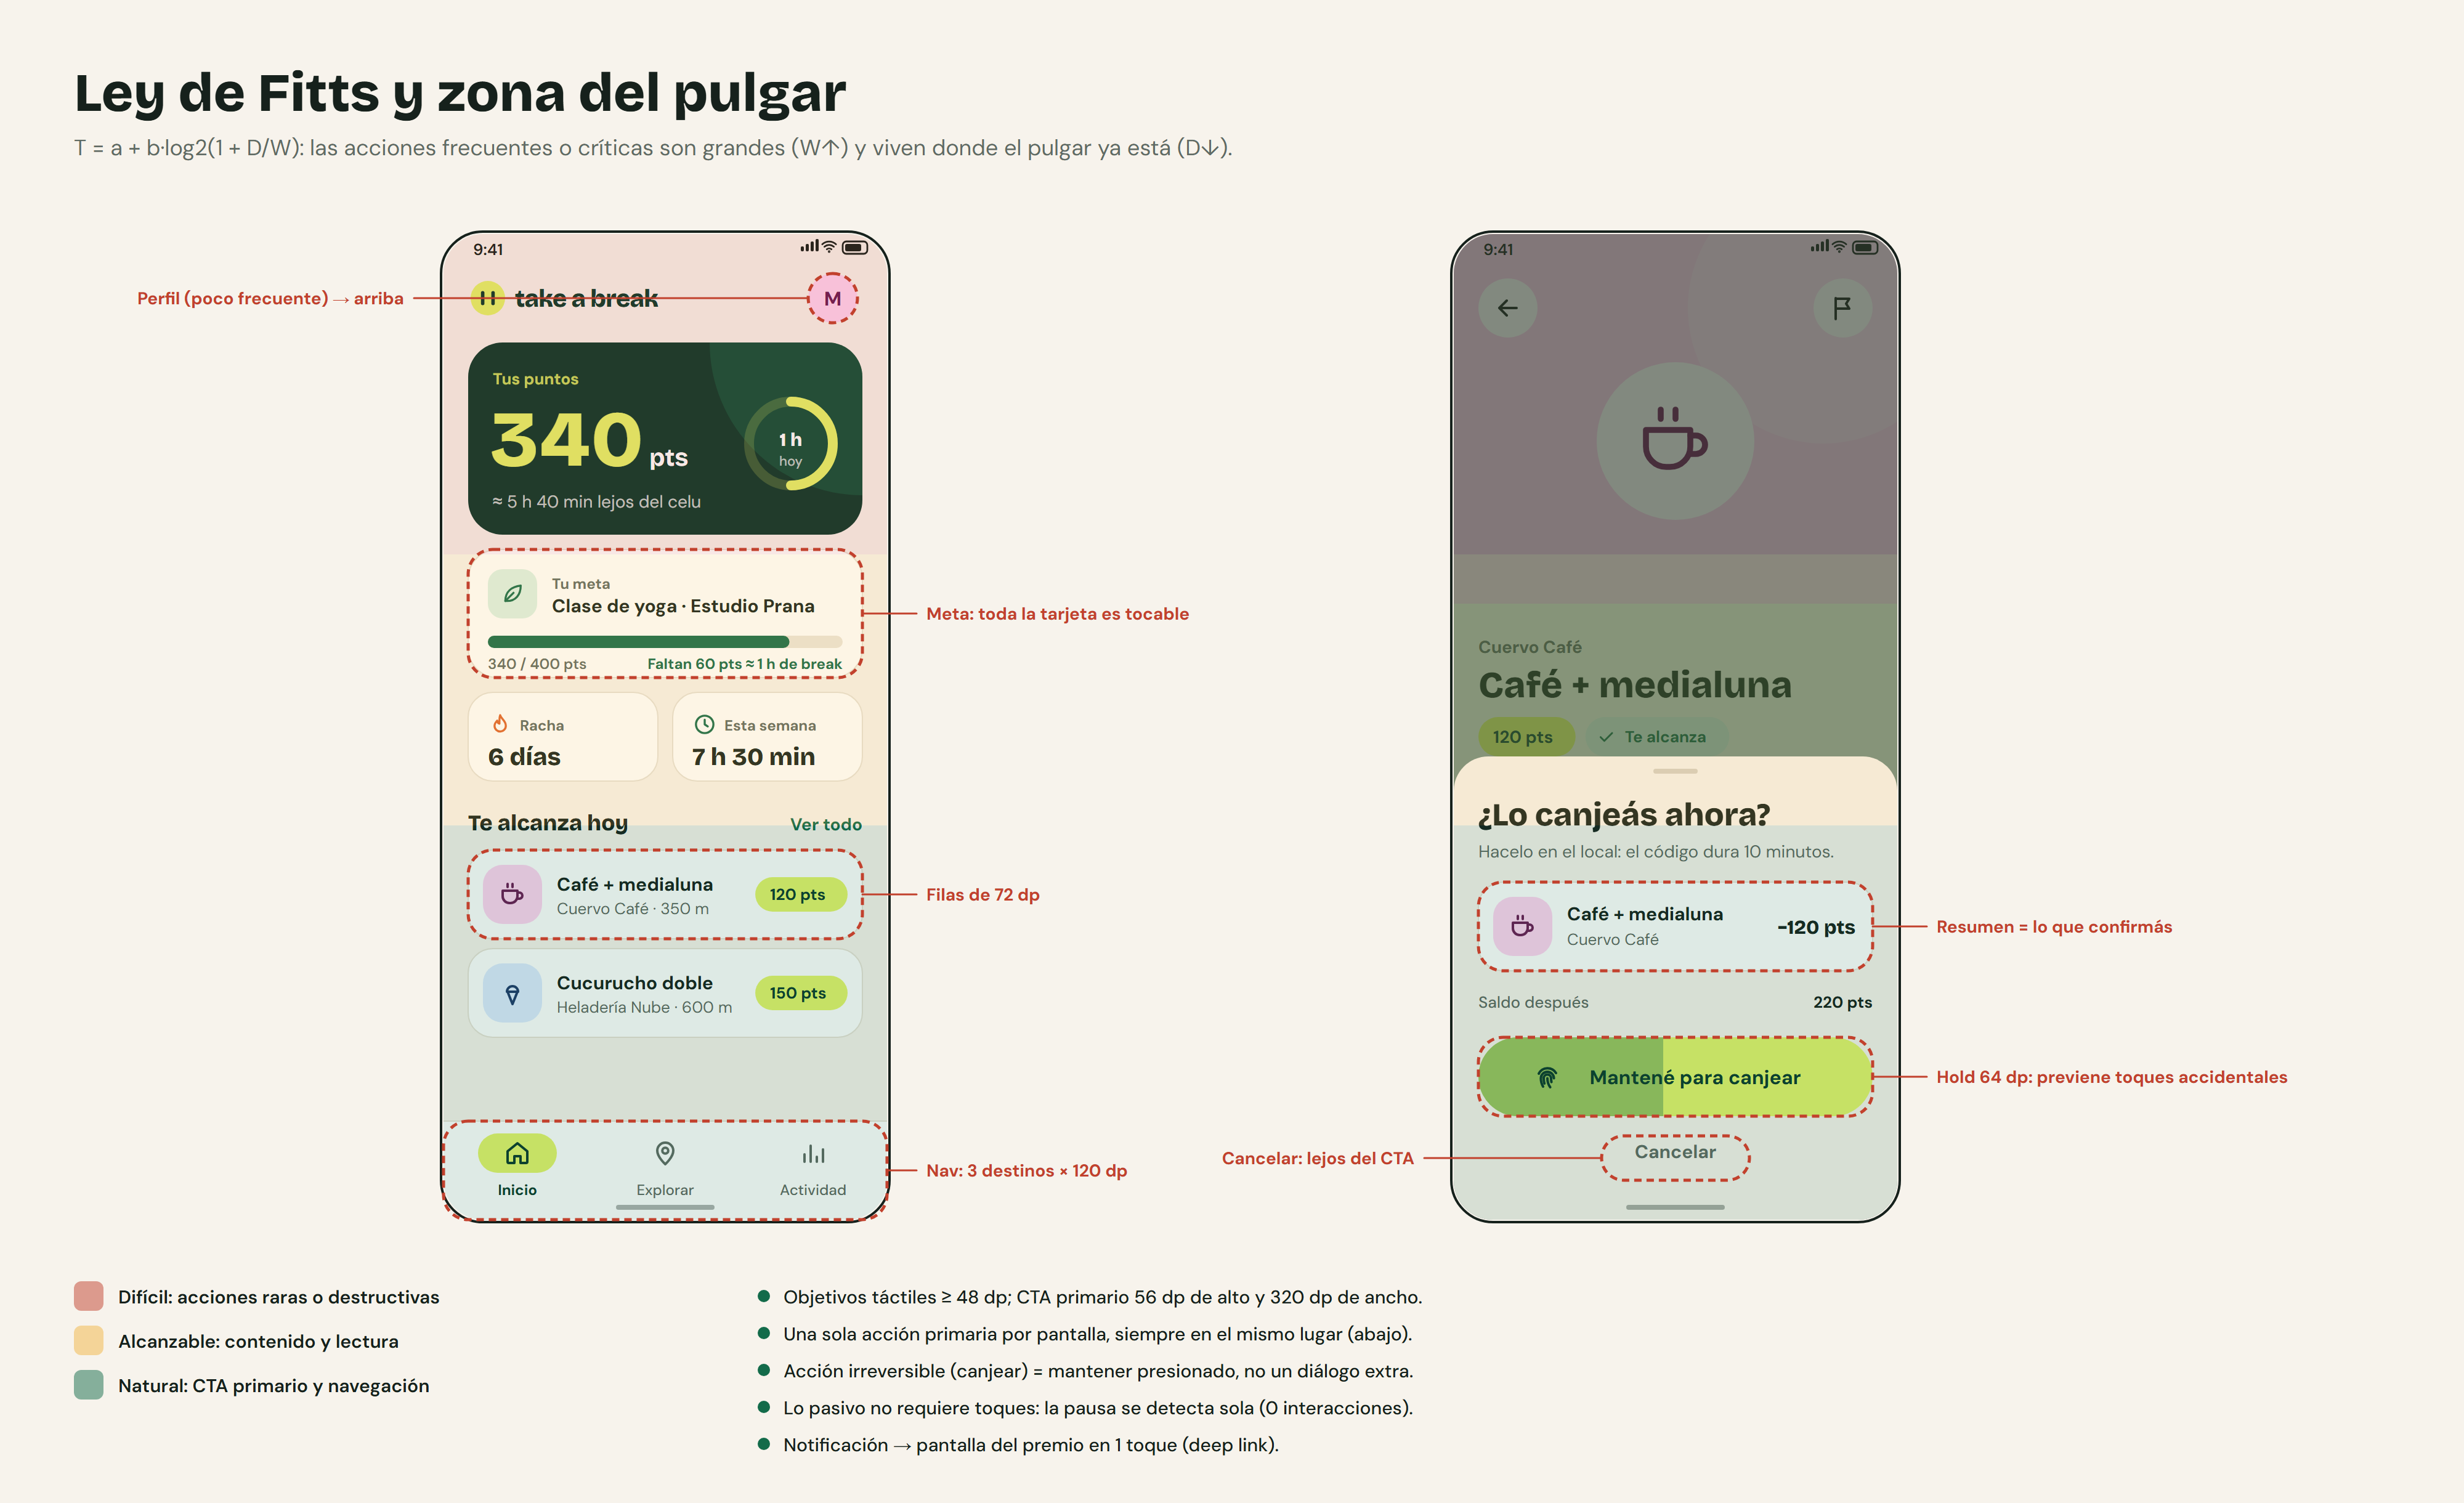
\includegraphics[width=\textwidth]{00-fitts-zona-pulgar.png}
\caption{Zona del pulgar sobre Inicio y la confirmación de canje. En rojo, los objetivos táctiles.}
\end{figure}

Medimos la fricción contando interacciones por tarea:

\begin{table}[H]
\centering\small
\begin{tabularx}{\textwidth}{@{}L l L@{}}
\toprule
\textbf{Tarea} & \textbf{Interacciones} & \textbf{Cómo} \\
\midrule
Registrar una pausa & 0 & Detección pasiva. \\
Ver cuánto sumó & 1 toque & Tocar la notificación. \\
Canjear un premio que alcanza & 2 toques y mantener & Fila del premio, Canjear, mantener. \\
Recuperar un código ya generado & 3 toques & Avatar, Mis canjes, Mostrar. \\
Fijar una meta & 2 toques & Premio, Fijar como meta. \\
\bottomrule
\end{tabularx}
\end{table}

\subsection{Pantallas principales}

Diseñamos 27 pantallas de 360 $\times$ 800 dp. Estas son las del caso de uso principal. El número de cada una coincide con el nombre del frame en Figma.

\begin{figure}[H]
\centering
\pantalla{08-inicio}{08 · Inicio}\hfill
\pantalla{09-inicio-validado}{09 · Break validado}\hfill
\pantalla{13-explorar}{13 · Explorar}\hfill
\pantalla{17-detalle}{17 · Detalle}\\[10pt]
\pantalla{19-confirmar-canje}{19 · Confirmar}\hfill
\pantalla{20-codigo}{20 · Código}\hfill
\pantalla{21-canje-pendiente}{21 · Canje pendiente}\hfill
\pantalla{23-actividad}{23 · Actividad}
\caption{Pantallas del caso de uso principal.}
\end{figure}

\subsubsection{Componentes y jerarquía}
\begin{itemize}
\item \textbf{Tarjeta de saldo}: es lo primero que se ve. El número grande en lima responde “¿cuánto tengo?”. El anillo muestra el avance del día contra la meta diaria.
\item \textbf{Tarjeta de meta}: responde “¿cuánto me falta?”. Cuando alcanza, aparece ahí mismo el botón Canjear (pantalla 09).
\item \textbf{Fila de premio}: ícono, nombre, comercio, distancia y un chip con los puntos. El chip es lima si alcanza y gris si no.
\item \textbf{Hoja inferior de Explorar}: el mapa orienta, pero la lista (abajo, al alcance del pulgar) es la que se toca.
\end{itemize}

\subsubsection{Estados}

La consigna pide representar carga, contenido, vacío, error y offline. La tabla indica qué frame cubre cada caso.

\begin{table}[H]
\centering\small
\begin{tabularx}{\textwidth}{@{}l L L L L L@{}}
\toprule
\textbf{Pantalla} & \textbf{Carga} & \textbf{Contenido} & \textbf{Vacío} & \textbf{Error} & \textbf{Offline} \\
\midrule
Primer uso & 01 & 02 a 06 & & 07 (permiso rechazado) & \\
Inicio     & 11 & 08, 09 & 10 & No aplica, datos locales & 12 \\
Explorar   & Igual que 11 & 13 & & 14 (sin ubicación), 16 & 15 \\
Canje      & 19 (mantener) & 17, 18, 20 & & 22 (sin stock) & 21 \\
Actividad  & Igual que 11 & 23 & 24 & No aplica, datos locales & 23 \\
Perfil     & & 25, 26 & & & 26 (pendiente) \\
\bottomrule
\end{tabularx}
\end{table}

\subsection{Flujo de pantallas}

El diagrama de la página siguiente muestra el punto de entrada, las decisiones y los finales posibles:

\begin{itemize}
\item \textbf{Primer uso (A).} Splash, onboarding, acceso y permisos. La decisión es si el usuario da el acceso a uso. Si no lo da, puede reintentar o entrar igual a ver premios.
\item \textbf{Ciclo principal (B).} Las flechas punteadas son transiciones del sistema. WorkManager lee los eventos, valida la pausa y, si es válida, notifica. Desde ahí el usuario llega al premio, confirma y, según haya conexión, obtiene el código o queda pendiente. El recorrido termina con el canje en el local o con los puntos devueltos.
\item \textbf{Navegación (C).} Tres pestañas más el perfil desde el avatar.
\end{itemize}

\begin{landscape}
\begin{figure}[p]
\centering
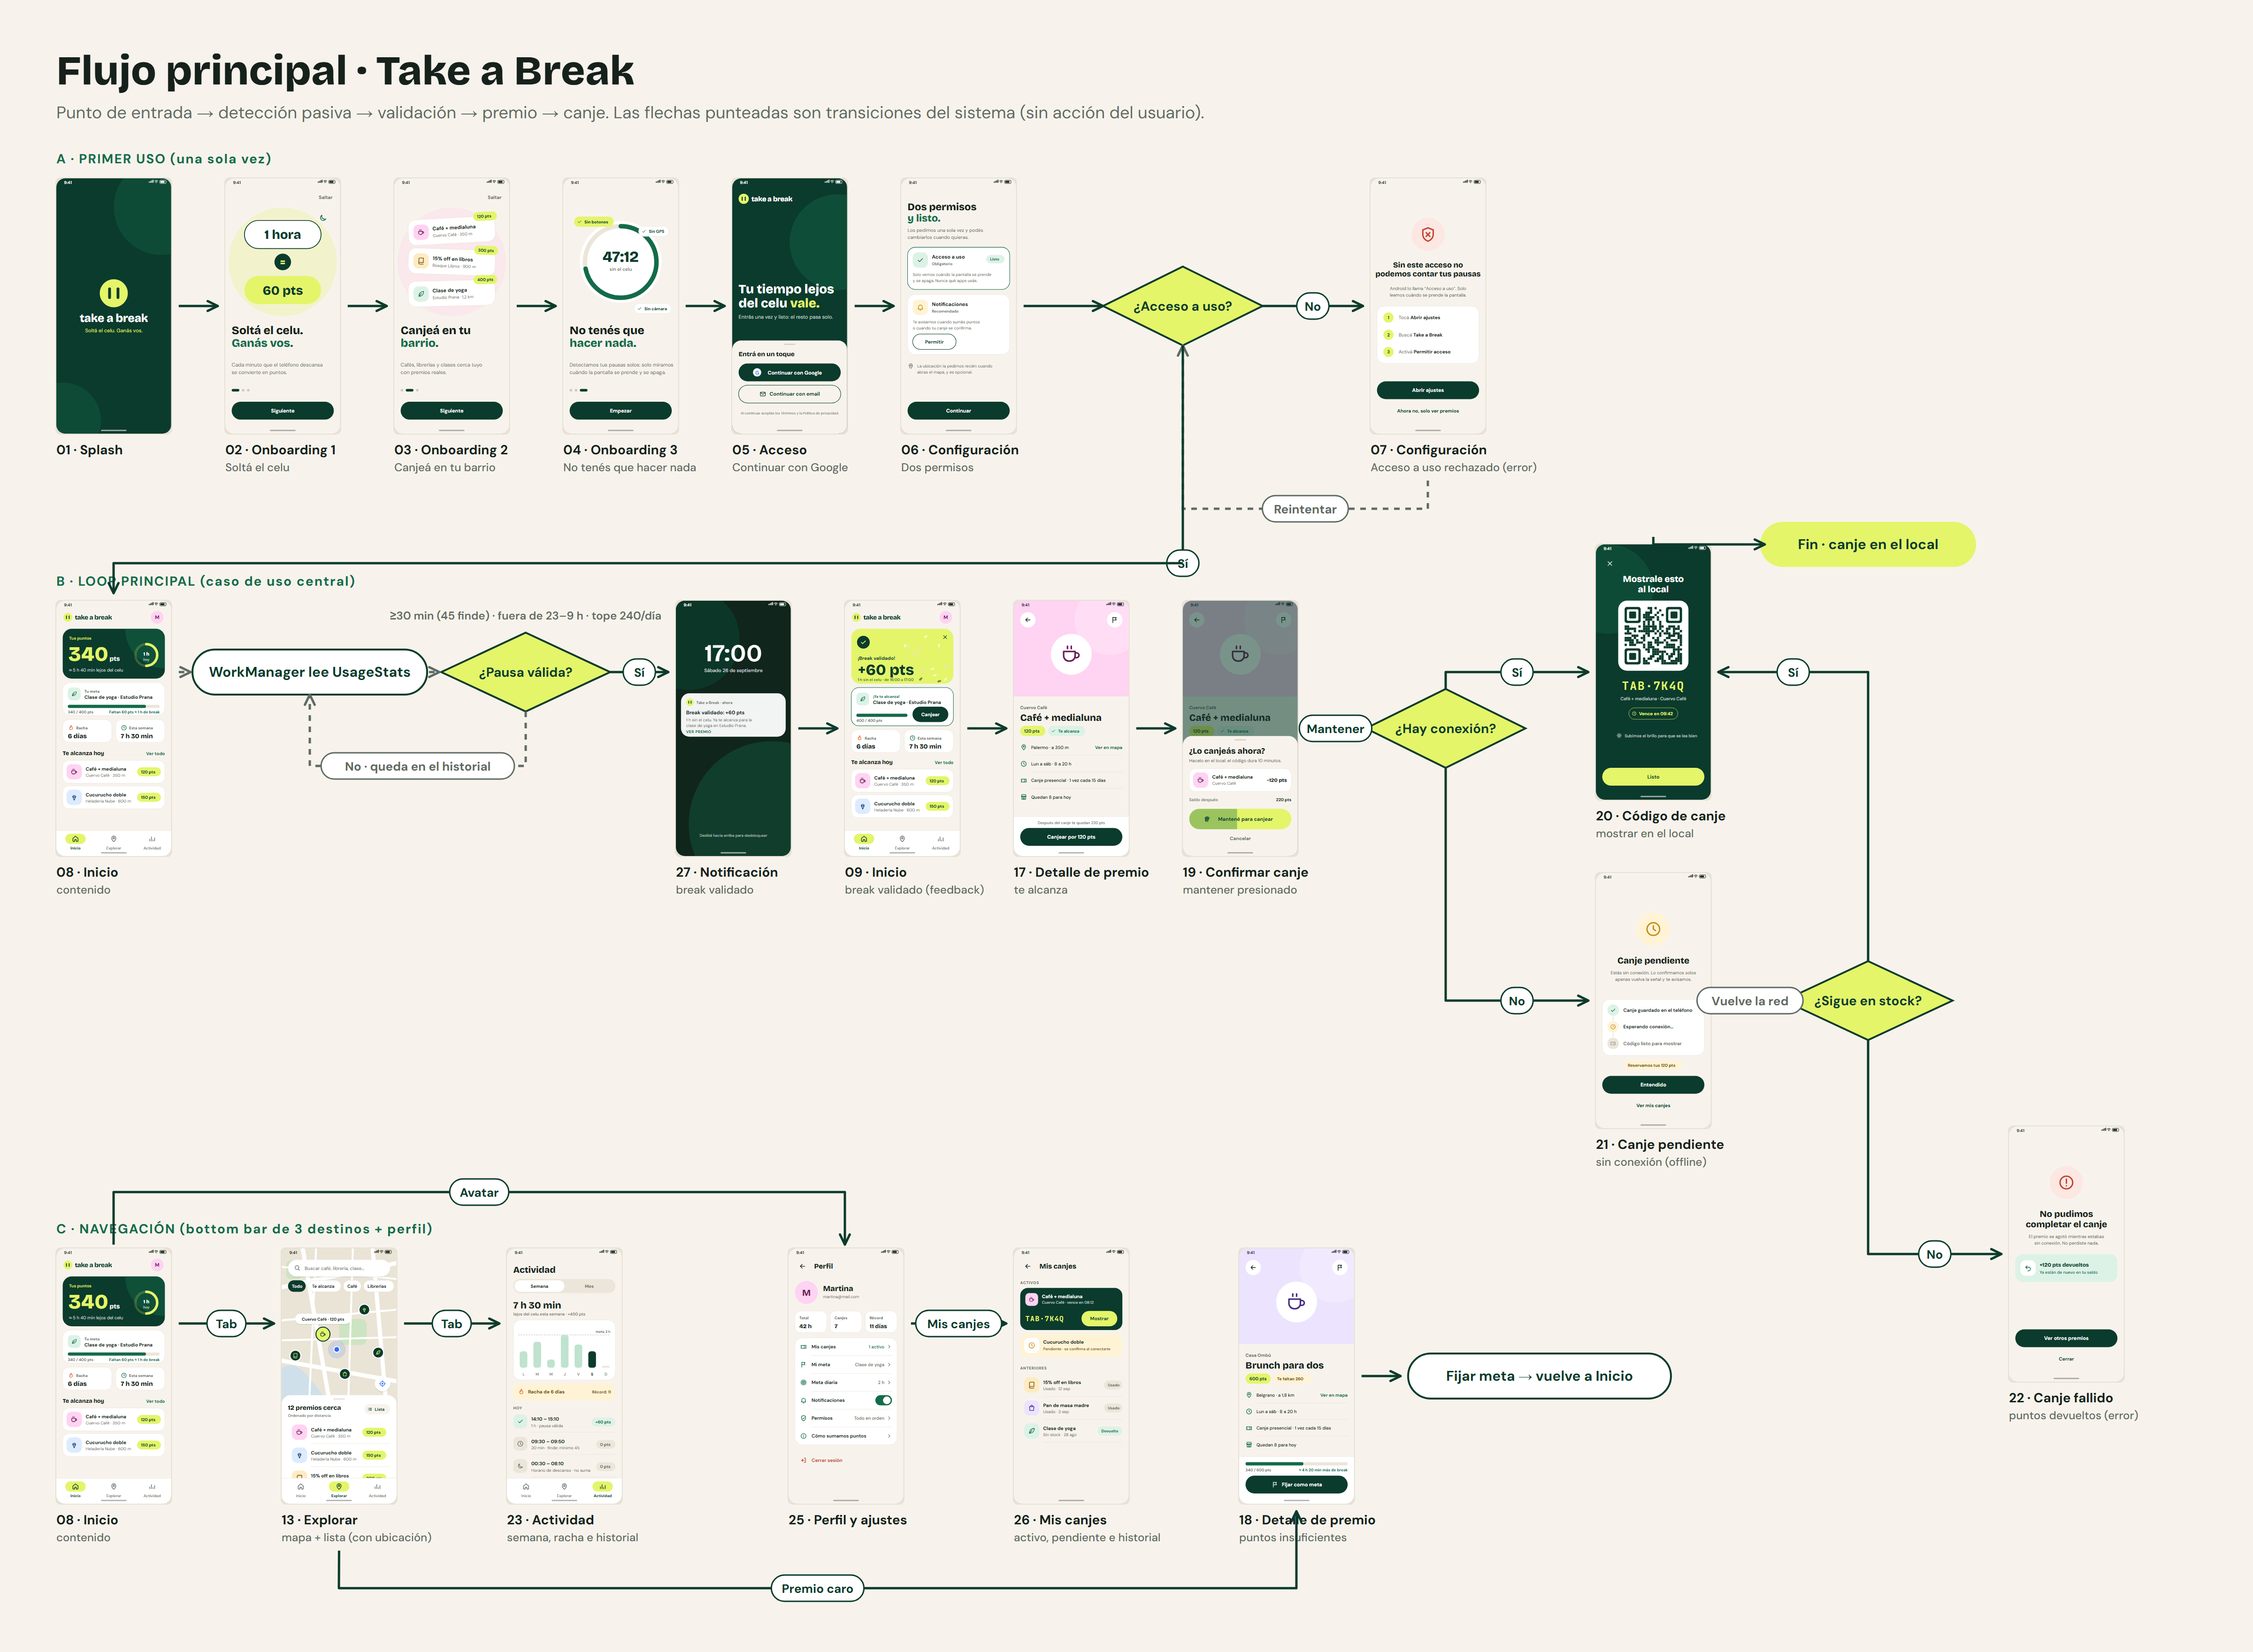
\includegraphics[width=\linewidth]{00-flujo-principal.png}
\caption{Flujo principal de interacción.}
\end{figure}
\end{landscape}

\section{Testear: plan de validación}
\label{sec:testear}

Todavía no probamos el diseño con usuarios. Antes de empezar a programar vamos a hacer dos validaciones.

\textbf{1. Prueba del prototipo.} Con cinco personas del perfil de la sección~\ref{sec:empatizar} y el prototipo navegable de Figma. Primero una entrevista corta sobre cómo intentaron usar menos el celular. Después, cuatro tareas:

\begin{enumerate}[label=T\arabic*.]
\item Entender cómo se ganan puntos sin que nadie lo explique.
\item Encontrar un premio que ya alcance y canjearlo.
\item Decir por qué una pausa de anoche no sumó.
\item Canjear sin conexión y explicar qué pasó.
\end{enumerate}

Vamos a medir si completan cada tarea, el tiempo, la cantidad de toques y los errores, y al final aplicar el cuestionario SUS. Si dos de cinco personas no pueden completar una tarea, esa parte se rediseña antes de implementarla.

\textbf{2. Prueba técnica de la detección.} Una app mínima que lea los eventos de bloqueo con \texttt{UsageStatsManager} en tres dispositivos de marcas distintas y en el emulador. Sirve para confirmar que los eventos llegan completos antes de apoyar todo el producto en ellos.

\section{Arquitectura}
\label{sec:arquitectura}

La app sigue MVVM con los principios de Clean Architecture. Las dependencias apuntan hacia el dominio: la UI conoce al ViewModel, el ViewModel a los casos de uso y los casos de uso solo conocen interfaces de repositorio. El dominio no importa nada de Android, así que las reglas de validación se prueban con tests unitarios comunes.

\subsection{Capas y responsabilidades}

\begin{table}[H]
\centering\small
\begin{tabularx}{\textwidth}{@{}l L@{}}
\toprule
\textbf{Capa} & \textbf{Qué contiene} \\
\midrule
Presentación & Pantallas en Jetpack Compose y un ViewModel por pantalla. Cada ViewModel expone un \texttt{StateFlow<UiState>} con los estados \textit{Loading}, \textit{Content}, \textit{Empty} y \textit{Error}, más una marca de offline. La UI no decide nada: dibuja el estado y envía eventos. \\
Dominio & Modelos (\texttt{BreakSession}, \texttt{Reward}, \texttt{Business}, \texttt{Redemption}), las reglas de validación (\texttt{BreakRules}), los casos de uso (\texttt{SyncBreaks}, \texttt{GetHomeSummary}, \texttt{GetRewards}, \texttt{RedeemReward}, \texttt{SetGoal}) y las interfaces de los repositorios. \\
Datos & Implementaciones de los repositorios, DAOs de Room, servicio Retrofit, DataStore y mappers entre entidades, DTOs y modelos. \\
Plataforma & Workers de WorkManager, lectura de eventos con \texttt{UsageStatsManager}, notificaciones y ubicación. Están detrás de interfaces para poder reemplazarlos en los tests. \\
\bottomrule
\end{tabularx}
\end{table}

\noindent\begin{minipage}{\linewidth}
\begin{lstlisting}
com.takeabreak
 |- ui/          screens, components, theme, navigation
 |- presentation/ viewmodels y UiState
 |- domain/      model, rules, usecase, repository (interfaces)
 |- data/        local (Room, DataStore), remote (Retrofit), repository, mapper
 |- platform/    workers, usage (UsageStatsManager), notifications, location
 |- di/          AppContainer (inyección manual)
\end{lstlisting}
\end{minipage}

La inyección de dependencias es manual, con un \texttt{AppContainer}. Para el tamaño del proyecto alcanza y evita sumar Hilt.

\subsection{Flujo de datos}

\begin{figure}[H]
\centering
\begin{tikzpicture}[
  node distance=7mm and 7mm,
  caja/.style={draw=bosque, fill=white, rounded corners=3pt, align=center, font=\footnotesize, minimum height=12mm, text width=22mm, line width=0.7pt},
  ext/.style={caja, fill=crema, draw=gris},
  capa/.style={font=\scriptsize\bfseries, text=verde},
  flecha/.style={-{Stealth[length=2.2mm]}, thick, bosque},
  vuelta/.style={-{Stealth[length=2.2mm]}, thick, verde, dashed},
  etq/.style={font=\scriptsize, fill=white, inner sep=1.5pt}
]
\node[caja] (ui) {UI\\Compose};
\node[caja, right=of ui] (vm) {ViewModel\\\texttt{StateFlow}};
\node[caja, right=of vm] (uc) {Casos de uso\\\texttt{BreakRules}};
\node[caja, right=of uc] (repo) {Repositorios};
\node[ext, right=of repo, yshift=10mm] (room) {Room\\(fuente local)};
\node[ext, right=of repo, yshift=-10mm] (api) {Retrofit\\API REST};

\node[caja, below=16mm of uc, text width=26mm] (worker) {WorkManager\\\texttt{BreakSyncWorker}};
\node[ext, left=15mm of worker, text width=28mm] (usage) {UsageStatsManager\\(Android)};
\node[ext, right=15mm of worker] (notif) {Notificación\\local};

\node[capa, above=2mm of ui.north east, xshift=4mm] {PRESENTACIÓN};
\node[capa, above=2mm of uc] {DOMINIO};
\node[capa, above=2mm of room] {DATOS};
\node[capa, below=2mm of worker] {PLATAFORMA};

\draw[flecha] (ui) to node[etq, above=1mm] {evento} (vm);
\draw[flecha] (vm) to (uc);
\draw[flecha] (uc) to (repo);
\draw[flecha] (repo) to (room);
\draw[flecha] (repo) to (api);

\draw[vuelta] (room.north) |- ++(0,7mm) -| node[etq, pos=0.25, above=1mm] {Flow: cuando Room cambia, la UI se recompone sola} (ui.north);

\draw[flecha] (worker) to node[etq, above=1mm] {1. lee} (usage);
\draw[flecha] (worker) to node[etq, right] {2. valida y guarda} (uc);
\draw[flecha] (worker) to node[etq, above=1mm] {3. avisa} (notif);
\end{tikzpicture}
\caption{Flujo de datos. La línea punteada es el camino de vuelta reactivo.}
\end{figure}

Room es la única fuente de verdad. La UI nunca lee de la red: la red actualiza Room y Room avisa a la UI por \texttt{Flow}. Por eso la app se ve igual con o sin conexión.

\subsection{Cómo se detecta una pausa}

\begin{enumerate}
\item \texttt{BreakSyncWorker} corre cada 15 minutos (el mínimo de WorkManager) y también al abrir la app.
\item Pide a \texttt{UsageStatsManager} los eventos desde el último \textit{checkpoint} guardado en DataStore. Solo usa cuatro tipos: pantalla encendida, pantalla apagada, pantalla bloqueada y desbloqueada.
\item Arma las pausas cerradas: desde que se bloquea hasta que se desbloquea. Si la pantalla se enciende por una notificación y se vuelve a apagar sin desbloquear, la pausa sigue.
\item \texttt{BreakRules} calcula los puntos, se guarda todo en Room en una transacción junto con el nuevo checkpoint y, si sumó, se muestra la notificación.
\end{enumerate}

Como el checkpoint se guarda en la misma transacción, si el proceso muere a la mitad no se pierde ni se duplica ninguna pausa. Las reglas quedan en una función pura:

\noindent\begin{minipage}{\linewidth}
\begin{lstlisting}
object BreakRules {
    const val DAILY_CAP = 240

    fun points(pause: Pause, pointsToday: Int): Int {
        val minMinutes = if (pause.isWeekend) 45 else 30
        val countable = pause.minutesOutside(restFrom = 23, restTo = 9)
        if (countable < minMinutes) return 0
        return countable.coerceAtMost(DAILY_CAP - pointsToday)
    }
}
\end{lstlisting}
\end{minipage}

\subsection{Topología de infraestructura}

\begin{figure}[H]
\centering
\begin{tikzpicture}[
  caja/.style={draw=bosque, fill=white, rounded corners=3pt, align=center, font=\footnotesize, minimum height=10mm, text width=29mm, line width=0.7pt},
  so/.style={caja, fill=crema, draw=gris},
  grupo/.style={draw=bosque, rounded corners=6pt, inner sep=4mm, line width=0.8pt},
  titulo/.style={font=\scriptsize\bfseries, text=verde},
  flecha/.style={{Stealth[length=2.2mm]}-{Stealth[length=2.2mm]}, thick, bosque},
  etq/.style={font=\scriptsize, fill=white, inner sep=1.5pt}
]
% teléfono
\node[caja] (app) at (0,0) {App Take a Break\\Compose + ViewModels};
\node[caja] (room) at (0,-1.5) {Room (SQLite)\\pausas, catálogo, canjes};
\node[caja] (ds) at (0,-3.0) {DataStore\\preferencias, checkpoint};
\node[so] (wm) at (3.3,0) {WorkManager};
\node[so] (usage) at (3.3,-1.5) {UsageStatsManager};
\node[so] (loc) at (3.3,-3.0) {Fused Location\\Notificaciones};
\node[so] (cred) at (3.3,-4.5) {Credential Manager};
\node[grupo, fit=(app)(ds)(wm)(cred)(room), label={[titulo]above:TELÉFONO ANDROID (API 28+)}] (tel) {};

% nube del equipo
\node[caja] (ktor) at (10,0) {API REST\\Ktor};
\node[caja] (pg) at (10,-1.5) {PostgreSQL\\comercios, premios, canjes};
\node[grupo, fit=(ktor)(pg), label={[titulo]above:BACKEND DEL EQUIPO}] (nube) {};

% google
\node[so] (maps) at (10,-4.0) {Google Maps\\(tiles del mapa)};
\node[so] (gid) at (10,-5.3) {Google Identity};
\node[grupo, draw=gris, fit=(maps)(gid), label={[titulo]above:SERVICIOS DE GOOGLE}] (goo) {};

\draw[flecha] (tel.east |- ktor) to node[etq, above=1mm] {HTTPS · JSON} (ktor.west);
\draw[flecha] (ktor) to (pg);
\draw[flecha] (tel.east |- maps) to node[etq, above=1mm] {HTTPS} (maps.west);
\draw[flecha] (tel.east |- gid) to node[etq, above=1mm] {token de Google} (gid.west);
\end{tikzpicture}
\caption{Topología. El teléfono funciona solo; la red se usa para el catálogo, los canjes, el mapa y el acceso.}
\end{figure}

El backend es una API REST propia, hecha en Ktor para usar el mismo lenguaje que la app, con PostgreSQL y desplegada en un servicio gratuito como Render. Expone pocos endpoints:

\begin{table}[H]
\centering\small
\begin{tabularx}{\textwidth}{@{}l L@{}}
\toprule
\textbf{Endpoint} & \textbf{Uso} \\
\midrule
\texttt{POST /auth/google} & Recibe el token de Google y devuelve un token de sesión. \\
\texttt{GET /rewards?since=} & Catálogo de comercios y premios. Con \texttt{since} devuelve solo lo que cambió. \\
\texttt{POST /redemptions} & Crea un canje. El teléfono manda un UUID propio, así un reintento no crea un canje duplicado. \\
\texttt{GET /redemptions/\{id\}} & Estado de un canje (activo, usado, vencido, rechazado). \\
\bottomrule
\end{tabularx}
\end{table}

\section{Persistencia y datos}
\label{sec:datos}

Hay dos tipos de datos. Las pausas y los canjes se generan en el teléfono. Los comercios y los premios vienen del backend y se guardan en Room como caché.

\begin{table}[H]
\centering\small
\begin{tabularx}{\textwidth}{@{}l L l l@{}}
\toprule
\textbf{Entidad} & \textbf{Campos principales} & \textbf{Origen} & \textbf{Dónde vive} \\
\midrule
\texttt{BreakSession} & id, inicio, fin, minutos válidos, puntos, estado (válida, corta, descanso, tope) & Teléfono & Room \\
\texttt{Business} & id, nombre, dirección, barrio, lat, lng, horario & API & Room (caché) \\
\texttt{Reward} & id, businessId, título, puntos, stock diario, actualizado & API & Room (caché) \\
\texttt{Redemption} & id (UUID), rewardId, puntos, código, estado (pendiente, activo, usado, vencido, devuelto), creado, vence & Teléfono y API & Room y servidor \\
\bottomrule
\end{tabularx}
\end{table}

\textbf{Relaciones.} Un comercio tiene muchos premios y un premio puede tener muchos canjes. Las pausas no se relacionan con nada.

\textbf{El saldo no se guarda.} Se calcula como la suma de los puntos de las pausas menos los puntos de los canjes que no fueron devueltos. Así no puede quedar desincronizado con el historial.

\textbf{DataStore} guarda lo que no es una tabla: el checkpoint de eventos, la meta elegida, la meta diaria, si las notificaciones están activas, la hora de la última sincronización y el token de sesión cifrado.

Las pausas no se suben al servidor. Además de ahorrar red, es una decisión de privacidad: el horario en que alguien deja el teléfono dice mucho de su rutina.

\section{Estrategia Offline First}
\label{sec:offline}

La detección de pausas no usa la red en ningún momento. Lo único que depende de la conexión es el catálogo, el mapa y la confirmación de canjes.

\begin{table}[H]
\centering\small
\begin{tabularx}{\textwidth}{@{}l L L@{}}
\toprule
\textbf{Situación} & \textbf{Qué hace la app} & \textbf{Qué ve el usuario} \\
\midrule
Tiene conexión & Actualiza el catálogo cada 6 h, y al abrir Explorar si pasó más de 1 h. Envía los canjes pendientes. & Todo normal. \\
Pierde conexión & Sigue detectando y sumando. Los canjes nuevos quedan pendientes con los puntos reservados. & Un aviso: “Sin conexión · tus pausas se siguen contando” (frames 12 y 15). \\
Recupera conexión & Un worker con la restricción de red envía los pendientes, con reintentos y espera exponencial. & Una notificación cuando el canje se confirma. \\
Datos viejos & Muestra el catálogo guardado. El stock se vuelve a validar en el servidor al canjear. & La hora de la última actualización. \\
Sin datos todavía & Solo puede pasar en Explorar la primera vez sin red. Inicio funciona igual. & Estado de error con Reintentar (frame 16). \\
\bottomrule
\end{tabularx}
\end{table}

\textbf{Conflictos.} Para el catálogo y el stock manda el servidor. Si un canje pendiente se rechaza porque el premio se agotó o se dio de baja, pasa a “devuelto”, los puntos vuelven al saldo y se avisa al usuario (frame 22). El UUID que genera el teléfono evita duplicados si un envío se reintenta.

\textbf{Mapa sin red.} Los marcadores salen de Room, pero el fondo del mapa necesita conexión. En ese caso se muestra solo la lista.

\section{Tecnologías previstas}
\label{sec:tecnologias}

\begin{table}[H]
\centering\small
\begin{tabularx}{\textwidth}{@{}l L@{}}
\toprule
\textbf{Tecnología} & \textbf{Para qué la usamos} \\
\midrule
Kotlin y Jetpack Compose & Stack de la materia. La UI declarativa simplifica dibujar los distintos estados de cada pantalla. \\
Material 3 & Componentes base sobre los que aplicamos nuestros colores y tipografías. \\
Navigation Compose & Tres pestañas, detalle, canje y perfil. Permite abrir el premio desde la notificación (deep link). \\
ViewModel, StateFlow y Coroutines & Estado que sobrevive a la rotación y trabajo asíncrono sin bloquear la UI. \\
Room & Fuente de verdad local: pausas, catálogo en caché y canjes. Es la base del offline first. \\
DataStore & Preferencias, checkpoint de eventos y token de sesión. \\
Retrofit, OkHttp y kotlinx.serialization & Comunicación con la API del equipo. \\
WorkManager & Lectura periódica de eventos, sincronización del catálogo y reintento de canjes. Sobrevive a reinicios del teléfono. \\
UsageStatsManager & Fuente de la detección. Requiere el permiso especial de acceso a uso, que el usuario da desde Ajustes. \\
Notificaciones (NotificationCompat) & Aviso de pausa validada y de canje confirmado. En Android 13 o superior se pide el permiso. \\
Maps Compose y Fused Location & Mapa de comercios y ubicación puntual, solo en primer plano. \\
Credential Manager & Acceso con Google en un toque. \\
JUnit, Turbine y Compose UI Test & Tests de reglas, ViewModels y pantallas. \\
Ktor y PostgreSQL (backend) & API propia en el mismo lenguaje, con datos semilla de comercios y premios. \\
\bottomrule
\end{tabularx}
\end{table}

\textbf{Permisos que pide la app:} acceso a uso (obligatorio para sumar puntos), notificaciones (recomendado) y ubicación aproximada o precisa mientras se usa la app (opcional). No pide ubicación en segundo plano, cámara ni contactos.

\section{Repositorio y equipo}
\label{sec:equipo}

\subsection{Repositorios}

\begin{table}[H]
\centering\small
\begin{tabularx}{\textwidth}{@{}l L@{}}
\toprule
Código de la app & \url{https://github.com/DesarrolloApps1/tpo-da1} \\
Documentación y diseño & \url{https://github.com/DesarrolloApps1/docs} (este documento y los archivos de Figma) \\
Backend & \pendiente{a crear} \\
\bottomrule
\end{tabularx}
\end{table}

\subsection{Forma de trabajo}

\begin{itemize}
\item \textbf{Ramas.} \texttt{main} tiene solo versiones entregables y está protegida. \texttt{dev} es la rama de integración. \texttt{tst} se usa para probar antes de pasar a \texttt{main}. Cada tarea se hace en \texttt{feature/<tema>}, que sale de \texttt{dev}.
\item \textbf{Commits.} Chicos y frecuentes, en español y con prefijo: \texttt{feat:}, \texttt{fix:}, \texttt{docs:}, \texttt{test:}, \texttt{refactor:}.
\item \textbf{Pull requests.} Un PR por funcionalidad hacia \texttt{dev}, con al menos una revisión de otro integrante y los tests pasando. Al cerrar un hito se pasa \texttt{dev} a \texttt{tst} y, después de probar, a \texttt{main}.
\item \textbf{Tareas.} Un issue por requisito o pantalla, organizados en un tablero de GitHub Projects.
\end{itemize}

\subsection{Integrantes, roles y responsabilidades}

Los roles no son exclusivos. Todos revisan código de otras áreas y tienen que poder explicar la app completa.

\begin{table}[H]
\centering\small
\begin{tabularx}{\textwidth}{@{}l l L L@{}}
\toprule
\textbf{Integrante} & \textbf{Rol principal} & \textbf{Responsabilidades} & \textbf{Participa en} \\
\midrule
\pendiente{Nombre} & Arquitectura e integración & Estructura de capas, navegación, AppContainer, revisión de PRs & Todas las áreas \\
\pendiente{Nombre} & UI y UX & Diseño en Figma, tema de Compose, pantallas y estados, accesibilidad & Pruebas con usuarios \\
\pendiente{Nombre} & Datos y sincronización & Room, DataStore, Retrofit, backend y estrategia offline & Canje \\
\pendiente{Nombre} & Detección y plataforma & Worker, UsageStatsManager, reglas de validación, notificaciones & Testing \\
\pendiente{Nombre} & Testing y documentación & Tests unitarios y de UI, README, este documento & Todas las áreas \\
\bottomrule
\end{tabularx}
\end{table}

\textbf{Cambios en el equipo:} \pendiente{ninguno hasta la fecha}.

\appendix
\newpage
\section{Todas las pantallas}
\label{anx:pantallas}

Cada frame se nombra con su número. Los archivos editables están en \texttt{docs/figma/screens}.

\subsection*{A · Primer uso}
\begin{figure}[H]
\centering
\pantalla{01-splash}{01 · Splash}\hfill
\pantalla{02-onboarding-1}{02 · Onboarding 1}\hfill
\pantalla{03-onboarding-2}{03 · Onboarding 2}\hfill
\pantalla{04-onboarding-3}{04 · Onboarding 3}\\[10pt]
\pantalla{05-acceso}{05 · Acceso}\hfill
\pantalla{06-permisos}{06 · Permisos}\hfill
\pantalla{07-permiso-rechazado}{07 · Permiso rechazado}\hfill
\begin{minipage}[t]{0.235\textwidth}\end{minipage}
\end{figure}

\subsection*{B · Inicio}
\begin{figure}[H]
\centering
\pantalla{08-inicio}{08 · Contenido}\hfill
\pantalla{09-inicio-validado}{09 · Break validado}\hfill
\pantalla{10-inicio-vacio}{10 · Vacío}\hfill
\pantalla{11-inicio-cargando}{11 · Cargando}\\[10pt]
\pantalla{12-inicio-offline}{12 · Sin conexión}\hfill
\begin{minipage}[t]{0.235\textwidth}\end{minipage}\hfill
\begin{minipage}[t]{0.235\textwidth}\end{minipage}\hfill
\begin{minipage}[t]{0.235\textwidth}\end{minipage}
\end{figure}

\subsection*{C · Explorar}
\begin{figure}[H]
\centering
\pantalla{13-explorar}{13 · Mapa y lista}\hfill
\pantalla{14-explorar-sin-ubicacion}{14 · Sin ubicación}\hfill
\pantalla{15-explorar-offline}{15 · Sin conexión}\hfill
\pantalla{16-explorar-error}{16 · Error sin datos}
\end{figure}

\subsection*{D · Canje}
\begin{figure}[H]
\centering
\pantalla{17-detalle}{17 · Detalle}\hfill
\pantalla{18-detalle-insuficiente}{18 · No alcanza}\hfill
\pantalla{19-confirmar-canje}{19 · Confirmar}\hfill
\pantalla{20-codigo}{20 · Código}\\[10pt]
\pantalla{21-canje-pendiente}{21 · Pendiente}\hfill
\pantalla{22-canje-fallido}{22 · Fallido}\hfill
\begin{minipage}[t]{0.235\textwidth}\end{minipage}\hfill
\begin{minipage}[t]{0.235\textwidth}\end{minipage}
\end{figure}

\subsection*{E · Actividad, F · Perfil y G · Sistema}
\begin{figure}[H]
\centering
\pantalla{23-actividad}{23 · Actividad}\hfill
\pantalla{24-actividad-vacia}{24 · Actividad vacía}\hfill
\pantalla{25-perfil}{25 · Perfil}\hfill
\pantalla{26-mis-canjes}{26 · Mis canjes}\\[10pt]
\pantalla{27-notificacion}{27 · Notificación}\hfill
\begin{minipage}[t]{0.235\textwidth}\end{minipage}\hfill
\begin{minipage}[t]{0.235\textwidth}\end{minipage}\hfill
\begin{minipage}[t]{0.235\textwidth}\end{minipage}
\end{figure}

\section{Sistema de diseño}
\label{anx:sistema}

\begin{figure}[H]
\centering
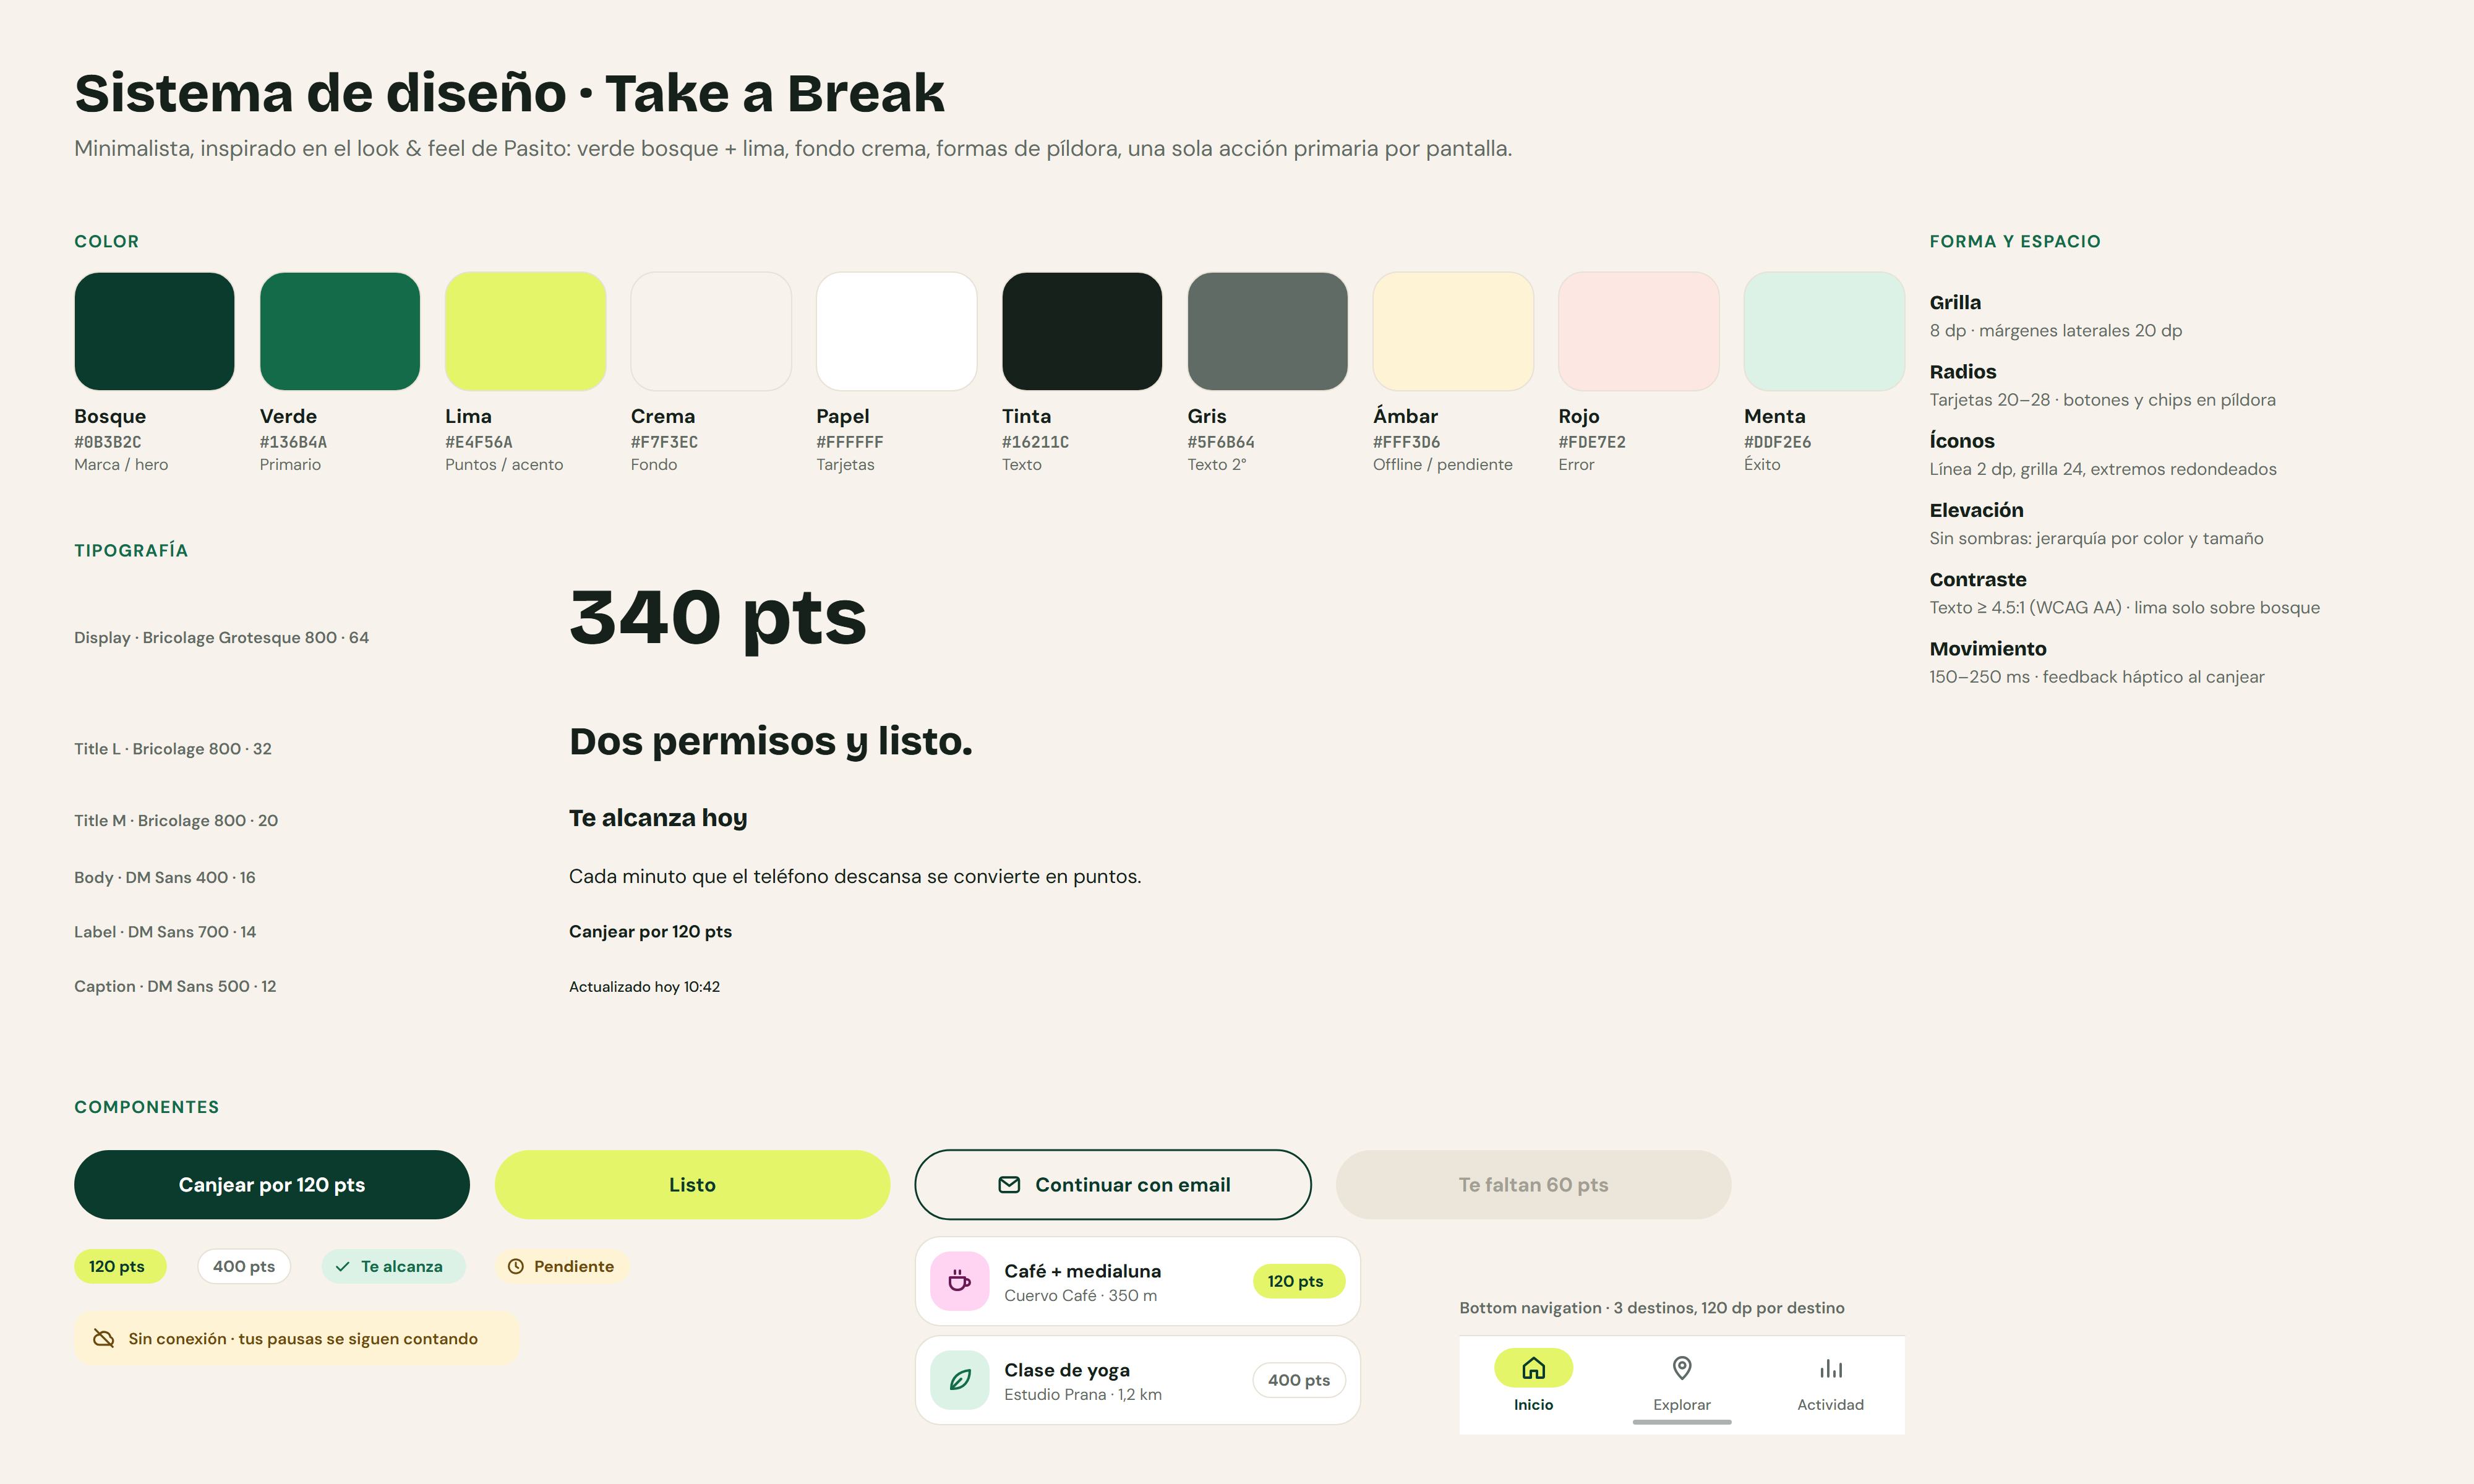
\includegraphics[width=\textwidth]{00-sistema-de-diseno.png}
\end{figure}

\section{Bocetos originales}
\label{anx:bocetos}

\begin{figure}[H]
\centering
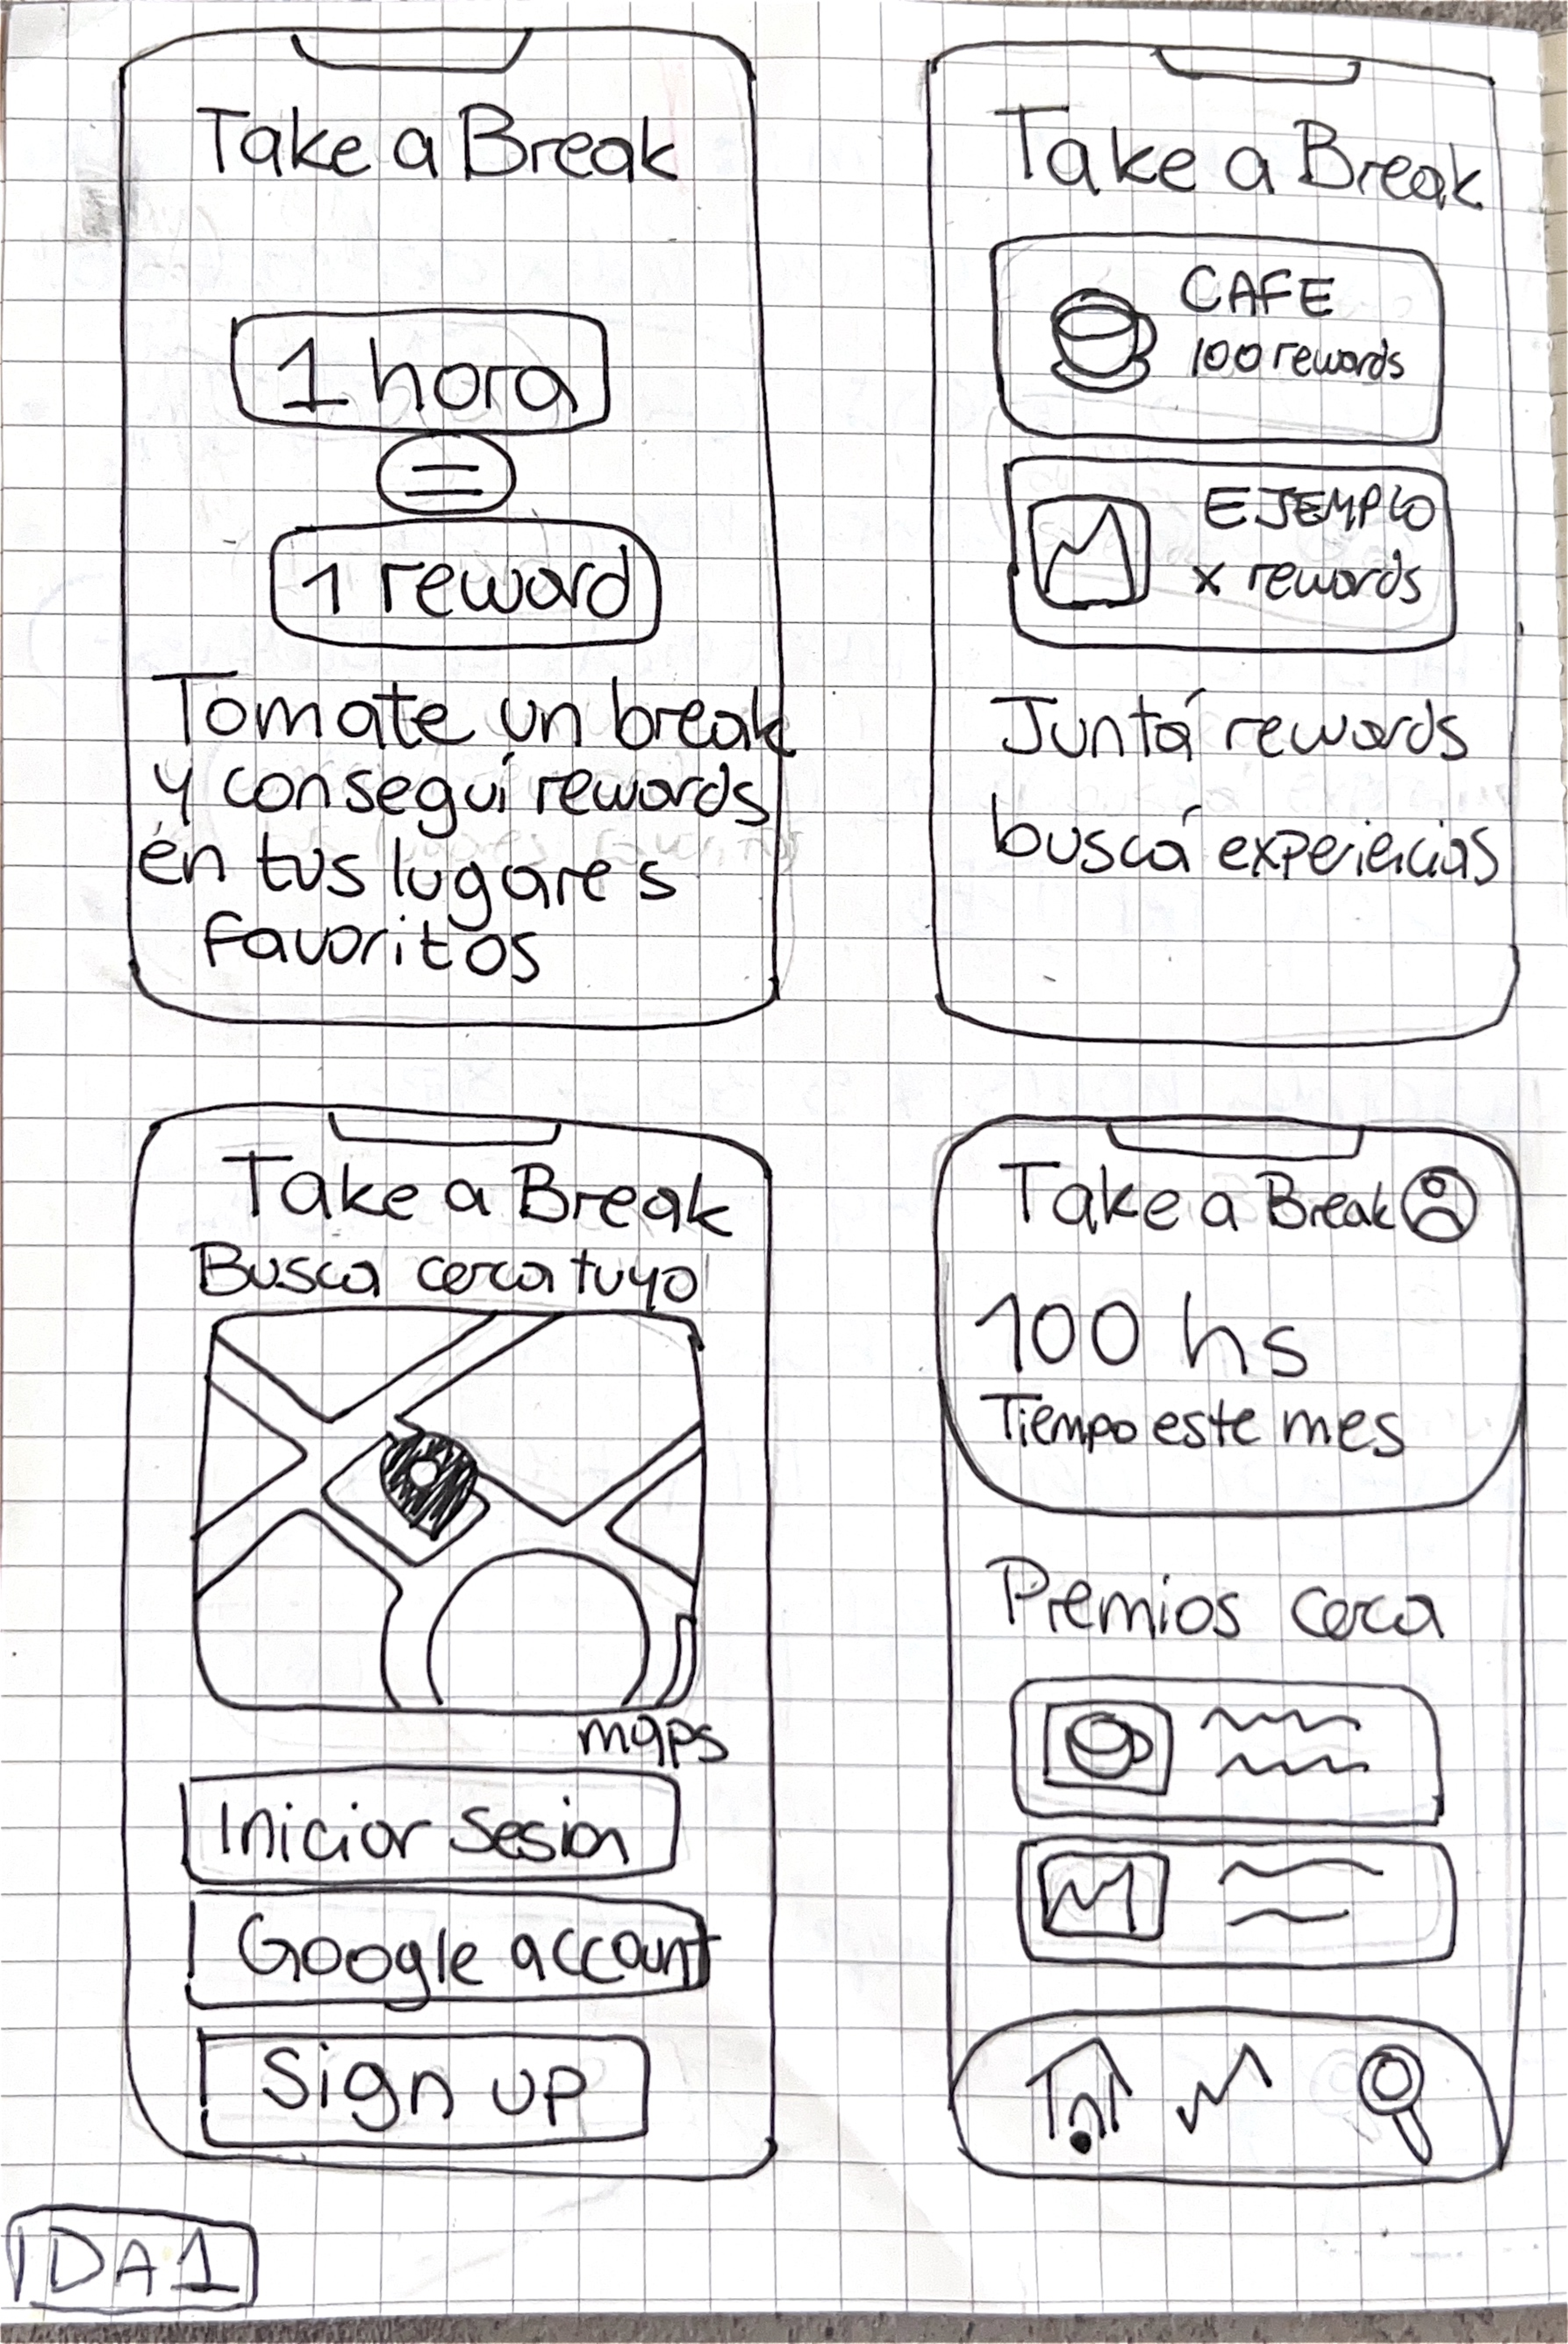
\includegraphics[page=1,height=0.4\textheight]{bocetos.pdf}\hfill
\includegraphics[page=2,height=0.4\textheight]{bocetos.pdf}
\caption{Primeros bocetos en papel.}
\end{figure}


\end{document}
